
\chapter{Benchmarks}
\section{Testing environment}
\paragraph{} In order to verify the efficiency of the translation and compare performance 
between JavaScript code output by the original Kotlin JS compiler and the Kotlin to Scala.js 
compiler, different Kotlin benchmarks were implemented.

\paragraph{} The benchmarks implemented for this evaluation are the following :

\begin{itemize}
 \item \textbf{DeltaBlue benchmark} This is an implementation of the incremental constraint 
solver algorithm of the same name. It will mainly benchmark the oriented object capabilities of the 
compiler.
 \item \textbf{Long Micro benchmark} This is a micro benchmark running binary operations on Longs.
 \item \textbf{Richards benchmark} This is a simulation of an operating system scheduler. It is 
mainly designed to test operations on arrays.
 \item \textbf{SHA512 benchmark} This is an implementation of SHA512 using Longs.
\end{itemize}

\paragraph{} The Kotlin to Scala.js compiler was used with the \scalainline{fullOpt} option set on 
the Scala.js linker. All optimizations available were therefore applied except for the Google 
Closure Compiler which was disabled. On the other hand, the Kotlin JS compiler was used with no 
particular options. %apply plugin: 'kotlin-dce-js' ???%

\paragraph{} Because the Kotlin standard library is not available yet, a simple LinkedList 
implementation was used to provide support for lists on both compilers. All benchmarks can 
be found inside the \scalainline{test/src/resources/src/benchmarks} folder of the GitHub
repository~\cite{kotlin_scalajs_v2}.

%\paragraph{Sudoku Solver}

\section{Results and analysis}

\paragraph{} The following results were obtained by compiling the benchmarks with both the Kotlin 
JS compiler and Kotlin to Scala.js. They were executed in a Linux Mint environment on two web 
browsers, namely Firefox 57.0.4 and Google Chrome 63.0.3239.132. Both browsers are 64-bit builds.

\paragraph{} Results for the LongMicro benchmark are presented after substraction of the LongNop result value. This means that the overhead time of computing anything else than an operation on Long values is not taken into account in the results.

\paragraph{} The raw data is presented in tables \ref{raw_firefox} and \ref{raw_chrome}. In order to better visualize the differences between the two compilers, data for DeltaBlue, Richards and SHA512 benchmarks were grouped in bar charts shown in figures \ref{chart_firefox} and \ref{chart_chrome}.

\begin{comment}
% bar chart with deltablue, richards and sha512
% richards tests integers and arrays of integers but scalajs keeps a wrapping of the arrays in 
order to keep to the  JVM implementation (so that we can do getClass and retrieve array of ints for 
example)
% try to identify why deltablue gives such a difference between firefox and chrome
%long micro --> substract the result of Nop from all other results
\end{comment}


\begin{figure*}[h]
    \centering
    
  \resizebox{0.9\textwidth}{!}{
    \begingroup
    \begin{subfigure}[h]{0.30\textwidth}
        \centering
        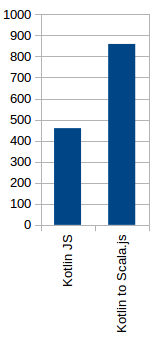
\includegraphics[height=8cm]{imgs/deltablue_barchart.png}
        \caption{DeltaBlue}
    \end{subfigure}
    ~
    \begin{subfigure}[h]{0.30\textwidth}
        \centering
        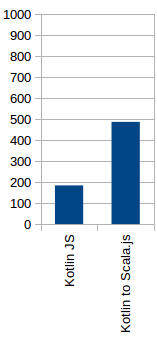
\includegraphics[height=8cm]{imgs/richards_barchart_firefox.png}
        \caption{Richards}
    \end{subfigure}
    ~
    \begin{subfigure}[h]{0.30\textwidth}
        \centering
        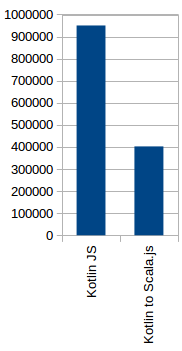
\includegraphics[height=8cm]{imgs/sha512_barchart_firefox.png}
        \caption{SHA512}
    \end{subfigure}
    \endgroup
  }
    
    \caption{Results in Firefox (lower is better)}
    \label{chart_firefox}
\end{figure*}


\begin{figure*}[h]
    \centering
    
  \resizebox{0.9\textwidth}{!}{
    \begingroup
    \begin{subfigure}[h]{0.30\textwidth}
        \centering
        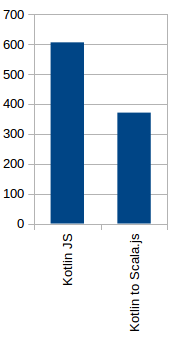
\includegraphics[height=8cm]{imgs/deltablue_barchart_chrome.png}
        \caption{DeltaBlue}
    \end{subfigure}
    ~
    \begin{subfigure}[h]{0.30\textwidth}
        \centering
        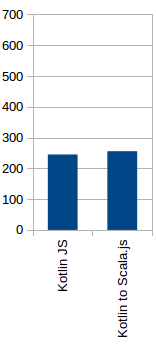
\includegraphics[height=8cm]{imgs/richards_barchart_chrome.png}
        \caption{Richards}
    \end{subfigure}
    ~
    \begin{subfigure}[h]{0.30\textwidth}
        \centering
        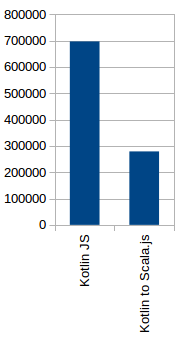
\includegraphics[height=8cm]{imgs/sha512_barchart_chrome.png}
        \caption{SHA512}
    \end{subfigure}
    \endgroup
  }
    
    \caption{Results in Google Chrome (lower is better)}
    \label{chart_chrome}
\end{figure*}


\begin{table}[htb]
  \centering
  \resizebox{\textwidth}{!}{
    \begingroup
    \renewcommand{\arraystretch}{1.5} % Default value: 1
    \begin{tabular}[c]{l | S[table-format=7.6] | S[table-format=4.6] | S[table-format=7.6] | S[table-format=5.6] |}
    & \multicolumn{2}{c|}{Kotlin JS} & \multicolumn{2}{c|}{Kotlin to Scala.js} \\ \hline
    
    Benchmark & \multicolumn{1}{c|}{Time ({$\mu$s})} & \multicolumn{1}{c|}{SEM} & \multicolumn{1}{c|}{Time ({$\mu$s})} & \multicolumn{1}{c|}{SEM} \\ \hline
    
    DeltaBlue & 459.28910 & 2.21871  & 859.11747 & 3.20804 \\
    
    LongMicro & & & & \\
    \multicolumn{1}{r|}{(LongNop)}    &   125.47639   &   0.70188 &   11.38803    &   0.02159 \\
    \multicolumn{1}{r|}{LongXor}    &   21.11297    &   0.77003 &   162.37052   &   0.56607 \\
    \multicolumn{1}{r|}{LongAdd}    &   165.33656   &   1.34534 &   198.32548   &   0.77713 \\
    \multicolumn{1}{r|}{LongMul}    &   2561.95739  &   4.75200 &   204.07814   &   0.63472 \\
    \multicolumn{1}{r|}{LongDiv32\_32}   &   6073.69372  &   28.94078    &   466.43548   &   1.08056 \\
    \multicolumn{1}{r|}{LongDiv32\_8}    &   8963.97814  &   14.92287    &   463.96042   &   1.00694 \\
    \multicolumn{1}{r|}{LongDiv53\_53}   &   5985.07349  &   26.34428    &   596.05268   &   1.27355 \\
    \multicolumn{1}{r|}{LongDiv53\_8}    &   9156.00966  &   72.35738    &   614.25587   &   1.59974 \\
    \multicolumn{1}{r|}{LongDiv64\_Pow2} &   9429.55544  &   18.06975    &   575.88860   &   1.01434 \\
    \multicolumn{1}{r|}{LongDiv64\_64}   &   5813.33312  &   13.79045    &   1028.32069  &   1.73338 \\
    \multicolumn{1}{r|}{LongDiv64\_8}    &   17033.25923 &   21.18046    &   1424.53345  &   2.37006 \\
    \multicolumn{1}{r|}{LongToString32} &   17519.93536 &   151.22958   &   552.06308   &   1.35633 \\
    \multicolumn{1}{r|}{LongToString53} &   28489.95217 &   250.54157   &   756.90514   &   5.21576 \\
    \multicolumn{1}{r|}{LongToString64} &   40159.85693 &   351.84462   &   3999.46757  &   33.08056    \\
    
    Richards & 184.11963 & 0.30823  & 487.24435 & 1.09796  \\
    SHA512 & 950152.00000 & 4554.93841 & 402408 & 8219.83114 \\
    \end{tabular}
    \endgroup
  }
  \caption{Results obtained in Firefox for both compilers}
  \label{raw_firefox}
\end{table}

\begin{table}[htb]
  \centering
  \resizebox{\textwidth}{!}{
    \begingroup
    \renewcommand{\arraystretch}{1.5} % Default value: 1
    \begin{tabular}[c]{l | S[table-format=7.6] | S[table-format=4.6] | S[table-format=7.6] | S[table-format=5.6] |}
    & \multicolumn{2}{c|}{Kotlin JS} & \multicolumn{2}{c|}{Kotlin to Scala.js} \\ \hline
    
    Benchmark & \multicolumn{1}{c|}{Time ({$\mu$s})} & \multicolumn{1}{c|}{SEM} & \multicolumn{1}{c|}{Time ({$\mu$s})} & \multicolumn{1}{c|}{SEM} \\ \hline
    
    DeltaBlue & 606.05524 & 1.78070 & 370.94092 & 1.52064 \\
    LongMicro & & & & \\
    \multicolumn{1}{r|}{(LongNop)}    &   95.09802    &   0.47985 &   43.68818    &   0.03876 \\
    \multicolumn{1}{r|}{LongXor}    &   154.29454   &   1.60520 &   132.63678   &   1.04405 \\
    \multicolumn{1}{r|}{LongAdd}    &   127.47245   &   1.58866 &   230.62637   &   2.32570 \\
    \multicolumn{1}{r|}{LongMul}    &   1061.11579  &   7.45646 &   228.63878   &   2.21889 \\
    \multicolumn{1}{r|}{LongDiv32\_32}   &   2808.60478  &   16.70720    &   462.99540   &   3.33924 \\
    \multicolumn{1}{r|}{LongDiv32\_8}    &   4144.76779  &   29.60327    &   445.63578   &   3.15253 \\
    \multicolumn{1}{r|}{LongDiv53\_53}   &   2704.16434  &   19.20949    &   513.25610   &   3.33351 \\
    \multicolumn{1}{r|}{LongDiv53\_8}    &   4481.03002  &   41.38667    &   499.07308   &   3.49403 \\
    \multicolumn{1}{r|}{LongDiv64\_Pow2} &   5165.94583  &   42.55326    &   490.20881   &   3.79047 \\
    \multicolumn{1}{r|}{LongDiv64\_64}   &   2804.60700  &   18.10513    &   849.86173   &   5.54424 \\
    \multicolumn{1}{r|}{LongDiv64\_8}    &   8631.07929  &   73.32333    &   1366.56581  &   6.29874 \\
    \multicolumn{1}{r|}{LongToString32} &   8129.34032  &   47.13448    &   504.82060   &   4.37917 \\
    \multicolumn{1}{r|}{LongToString53} &   13103.23530 &   93.32371    &   685.87353   &   6.50972 \\
    \multicolumn{1}{r|}{LongToString64} &   17988.75739 &   128.04266   &   1680.24284  &   8.84513 \\
	    
    Richards & 245.06567 & 0.49429 & 255.69825 & 0.52048 \\
	    
    SHA512 & 696866.00000 & 4694.32114 & 279157.5 & 11230.01427
    \end{tabular}
    \endgroup
  }
  
  \caption{Results obtained in Google Chrome for both compilers}
  \label{raw_chrome}
\end{table}

\begin{comment}
\paragraph{} As can be easily seen, the size of all output JavaScript code by the Kotlin to 
Scala.js compiler is significantly smaller. The major difference is due to the inclusion of the 
full Kotlin JS standard library with the generated code.
\end{comment}

\paragraph{} The results for the DeltaBlue benchmark are interesting. It seems that the implementation of the JavaScript runtime in both browsers differs at some point, leading Kotlin JS to perform better in Firefox whereas the Kotlin to Scala.js compiler has much better results in Google Chrome. It is hard to conclude which of the two compilers performed better here.

\paragraph{} Regarding the Richards benchmark, we can see that in Firefox Kotlin JS does better. This is probably because of the difference of translation of arrays between the two compilers. Scala.js keeps close to the JVM implementation of arrays and wraps all of them inside JavaScript classes. This requires a function call before obtaining the array itself and introduces execution overheads. This behavior allows to keep typing informations in the JavaScript code. Kotlin doesn't do that and therefore wins thanks to an implementation of arrays closer to JavaScript semantics.

\paragraph{} On the other hand, the execution times in Google Chrome are much closer. It is likely that this is of the same origin as for the DeltaBlue benchmark because of the indirection on array accesses.

\paragraph{} Both LongMicro and SHA512 benchmarks perform better with the Kotlin to Scala.js compiler in both web browsers. This large difference in performance is due to the optimized implementation of Longs in the Scala.js library and optimizer.
